\section{Технический проект}

\subsection{Общая характеристика организации решения задачи}

Разработанное веб-приложение представляет собой онлайн-платформу для самостоятельного изучения JavaScript иностранными студентами. Платформа реализована с использованием современных веб-технологий: HTML, CSS, JavaScript и Python (Django). Она размещается в сети Интернет (например, на домене (https://swsueducate.ru) и предоставляет единый пользовательский интерфейс для студентов и преподавателей.

Основные задачи платформы:
\begin{itemize}
	\item управление курсами и уроками;
	\item создание и проведение тестов;
	\item анализ результатов обучения;
	\item поддержка локализации для разных языков.
\end{itemize}

Система построена на клиент-серверной архитектуре:
\begin{enumerate}
	\item {Клиентская часть} (Frontend): Реализована с использованием HTML, CSS (Bootstrap для адаптивности) и JavaScript (включая Sortable.js для сортировки уроков). Отвечает за отображение интерфейса и интерактивность.
	\item {Серверная часть} (Backend): Построена на Django, обрабатывает запросы, управляет данными (через SQLite) и генерирует динамические страницы.
	\item {База данных}: SQLite хранит данные о курсах, уроках, тестах, пользователях и их прогрессе.
\end{enumerate}

\subsection{Архитектура системы}

Архитектура платформы следует модели MVC (Model-View-Controller), реализованной через Django, что обеспечивает чёткое разделение ответственности между компонентами системы. Описание архитектуры:

\begin{enumerate}
	\item {Model} (Модель): Определяет структуру данных в виде таблиц SQLite (courses\_course, courses\_lesson, courses\_test, courses\_question, courses\_answer, users\_user и др.). Модели Django обеспечивают взаимодействие с базой данных через ORM, упрощая операции создания, чтения, обновления и удаления данных (CRUD).
	\item {View} (Представление): Обрабатывает HTTP-запросы и формирует ответы. Включает функции и классы Django views, которые возвращают HTML-страницы (через шаблоны Django) или JSON-ответы для динамической загрузки данных.
	\item {Template} (Шаблоны): Реализован через маршрутизацию Django файл (urls.py), направляющую запросы к соответствующим представлениям.
\end{enumerate}

Основные компоненты системы:
\begin{enumerate}
	\item {Frontend}: Интерфейс пользователя, созданный с помощью шаблонов Django (HTML), стилей Bootstrap и JavaScript. Sortable.js используется для реализации сортировки уроков в интерфейсе преподавателя.
	\item {Backend}: Сервер Django, который управляет логикой приложения, включая аутентификацию (contrib.auth), ограничение доступа (@login\_required) и локализацию (i18n).
	\item {Database}: SQLite, содержащая реляционные таблицы для хранения данных. Использование SQLite обусловлено лёгкостью и достаточной производительностью для данного проекта.
	\item {API}: Внутренние API-методы (реализованы через Django views), обеспечивающие взаимодействие между клиентской и серверной частями, например, для загрузки списка уроков или результатов тестов.
\end{enumerate}

Архитектура представлена на диаграмме компонентов (см. рис.~\ref{diag:image}).
\newpage
\begin{figure}[h]
	\centering{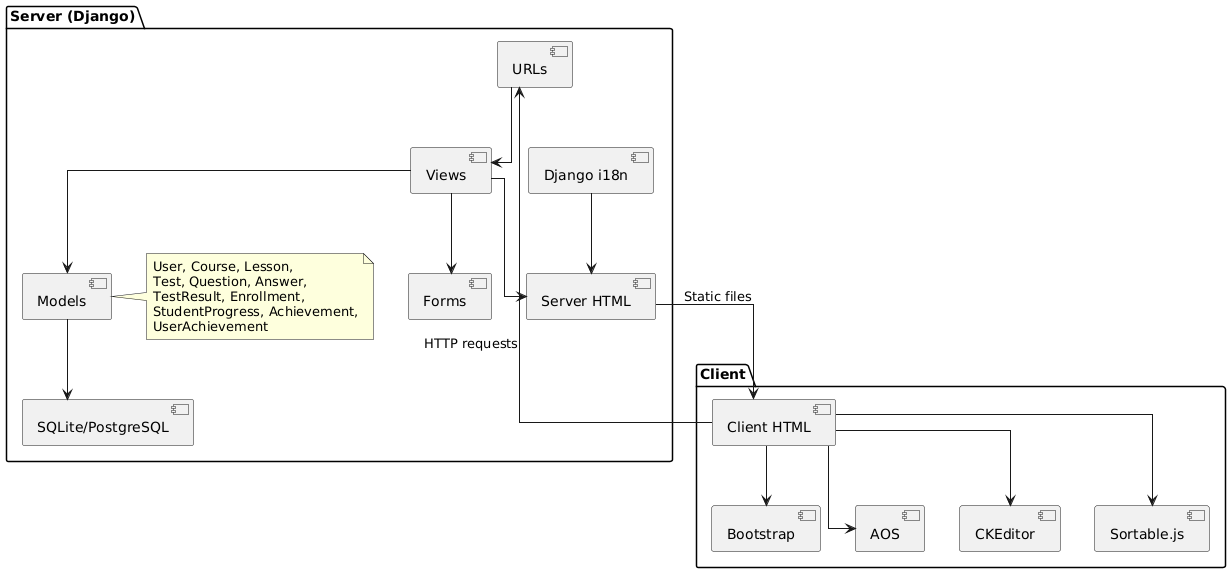
\includegraphics[width=1\linewidth]{images/диаграмма1}}
	\caption{Диаграмма компонентов}
	\label{diag:image}
\end{figure}

\subsection{Структура базы данных}

\subsubsection{Концептуальная модель данных}

На рисунке~\ref{conceptual_model} представлена концептуальная модель данных разрабатываемой обучающей платформы.

\begin{figure}[H]
	\centering
	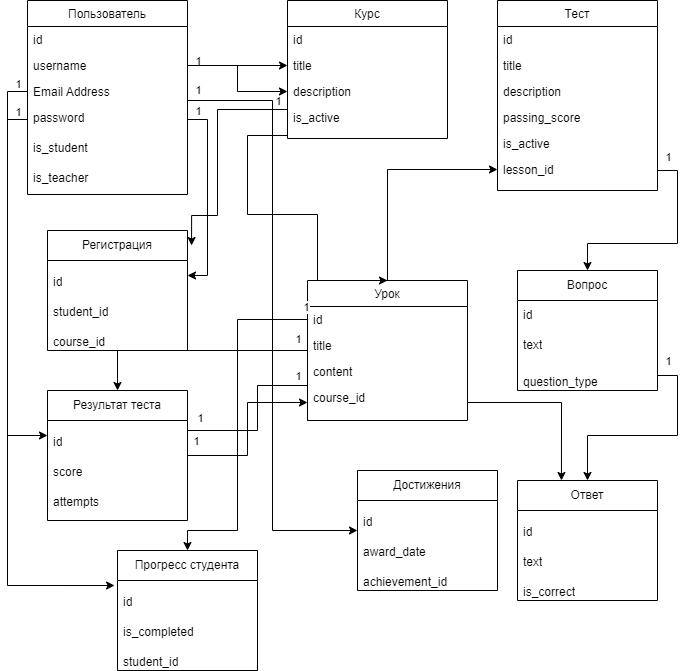
\includegraphics[width=0.95\textwidth]{images/концептуальная}
	\caption{Концептуальная модель данных обучающей платформы}
	\label{conceptual_model}
\end{figure}

Данная модель отражает основные сущности системы и связи между ними на логическом уровне.
Проанализировав требования, выделены следующие основные сущности:
\begin{itemize}
	\item курсы;
	\item уроки;
	\item тесты;
	\item вопросы;
	\item ответы;
	\item результаты тестов;
	\item пользователи;
	\item запись на курсы;
	\item прогресс;
	\item связь пользователей и курсов.
\end{itemize}

\subsubsection{Схема структуры базы данных}

На рисунке~\ref{bd:image} представлена схема структуры базы данных системы, отражающая таблицы, их атрибуты, ключи и связи между ними.

\begin{landscape}
	\begin{figure}[ht]
		\centering
		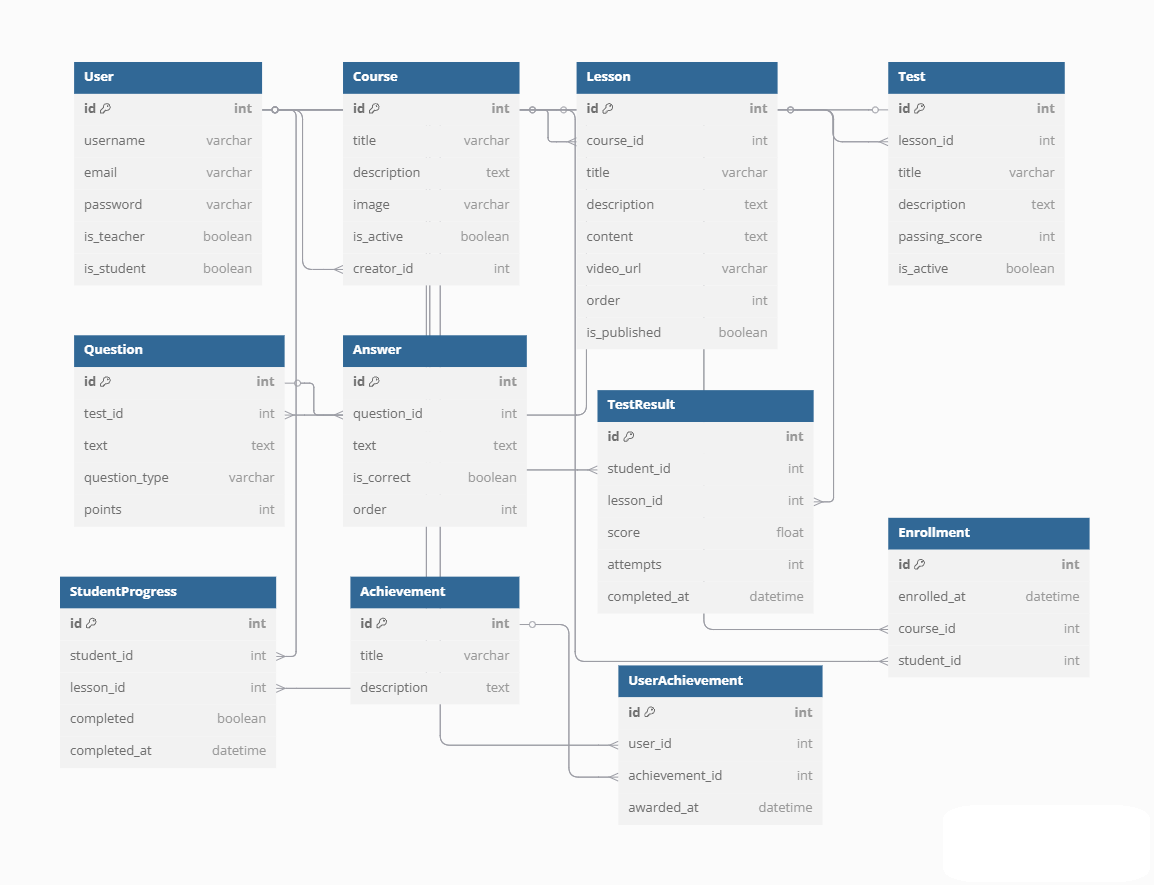
\includegraphics[width=1.3\textwidth]{images/бд} 
		\caption{Структура базы данных}
		\label{bd:image}
	\end{figure}
\end{landscape}

Ниже приведены атрибуты сущностей в формате таблиц.

\begin{xltabular}{\textwidth}{|l|l|p{3.2cm}|X|}
	\caption{Атрибуты сущности <<Курсы>>\label{courses:table}}\\ \hline
	Поле & Тип & Обязательное & Описание \\ \hline
	\endfirsthead
	\continuecaption{Продолжение таблицы \ref{courses:table}}\\ \hline
	Поле & Тип & Обязательное & Описание \\ \hline
	\endhead
	id & Integer & true & Уникальный идентификатор курса \\ \hline
	title & String & true & Название курса \\ \hline
	description & Text & true & Описание курса \\ \hline
	image & String & false & Путь к изображению курса \\ \hline
	isactive & Boolean & true & Признак активности курса \\ \hline
	createdat & DateTime & true & Дата создания курса \\ \hline
	teacherid & ForeignKey & true & Преподаватель (ссылка на таблицу Пользователи) \\ \hline
\end{xltabular}

\begin{xltabular}{\textwidth}{|l|l|p{3.2cm}|X|}
	\caption{Атрибуты сущности <<Уроки>>\label{lessons:table}}\\ \hline
	Поле & Тип & Обязательное & Описание \\ \hline
	\endfirsthead
	\continuecaption{Продолжение таблицы \ref{lessons:table}}\\ \hline
	Поле & Тип & Обязательное & Описание \\ \hline
	\endhead
	id & Integer & true & Уникальный идентификатор урока \\ \hline
	courseid & ForeignKey & true & Курс, к которому относится урок (ссылка на таблицу Курсы) \\ \hline
	title & String & true & Название урока \\ \hline
	description & Text & false & Описание урока \\ \hline
	content & Text & true & Содержимое урока (текст, HTML) \\ \hline
	videourl & String & true & Ссылка на видео урока \\ \hline
	order & Integer & true & Порядок урока в курсе \\ \hline
	ispublished & Boolean & true & Признак публикации урока \\ \hline
	createdat & DateTime & true & Дата создания урока \\ \hline
\end{xltabular}


\begin{xltabular}{\textwidth}{|l|l|p{3.2cm}|X|}
	\caption{Атрибуты сущности <<Тесты>>\label{tests:table}}\\ \hline
	Поле & Тип & Обязательное & Описание \\ \hline
	\endfirsthead
	\continuecaption{Продолжение таблицы \ref{tests:table}}\\ \hline
	Поле & Тип & Обязательное & Описание \\ \hline
	\endhead
	id & Integer & true & Уникальный идентификатор теста \\ \hline
	lessonid & ForeignKey & true & Урок, к которому относится тест (ссылка на таблицу Уроки) \\ \hline
	title & String & true & Название теста \\ \hline
	description & Text & true & Описание теста \\ \hline
	questions & Array & false & Список вопросов (JSON или связанные модели) \\ \hline
	isactive & Boolean & true & Признак активности теста \\ \hline
	passingscore & Integer & true & Проходной балл (в процентах) \\ \hline
	createdat & DateTime & false & Дата создания теста (может отсутствовать) \\ \hline
\end{xltabular}

\begin{xltabular}{\textwidth}{|l|l|p{3.2cm}|X|}
	\caption{Атрибуты сущности <<Результаты тестов>>\label{test_results:table}}\\ \hline
	Поле & Тип & Обязательное & Описание \\ \hline
	\endfirsthead
	\continuecaption{Продолжение таблицы \ref{test_results:table}}\\ \hline
	Поле & Тип & Обязательное & Описание \\ \hline
	\endhead
	id & Integer & true & Уникальный идентификатор результата \\ \hline
	studentid & ForeignKey & true & Студент (ссылка на таблицу Пользователи) \\ \hline
	lessonid & ForeignKey & true & Урок, связанный с тестом (ссылка на таблицу Уроки) \\ \hline
	score & Float & true & Оценка (в процентах или дробное значение) \\ \hline
	attempts & Integer & true & Количество попыток \\ \hline
	answers & Text & true & Ответы (в формате JSON) \\ \hline
	completedat & DateTime & true & Дата завершения теста \\ \hline
\end{xltabular}

\begin{xltabular}{\textwidth}{|l|l|p{3.2cm}|X|}
	\caption{Атрибуты сущности <<Пользователи>>\label{users:table}}\\ \hline
	Поле & Тип & Обязательное & Описание \\ \hline
	\endfirsthead
	\continuecaption{Продолжение таблицы \ref{users:table}}\\ \hline
	Поле & Тип & Обязательное & Описание \\ \hline
	\endhead
	id & Integer & true & Уникальный идентификатор пользователя \\ \hline
	username & String & true & Имя пользователя \\ \hline
	email & String & true & Электронная почта \\ \hline
	isteacher & Boolean & true & Признак преподавателя \\ \hline
	password & String & true & Хэшированный пароль пользователя \\ \hline
	lastlogin & DateTime & false & Дата последнего входа \\ \hline
	issuperuser & Boolean & true & Признак суперпользователя \\ \hline
	firstname & String & true & Имя пользователя \\ \hline
	lastname & String & true & Фамилия пользователя \\ \hline
	isstaff & Boolean & true & Признак персонала \\ \hline
	isactive & Boolean & true & Признак активности пользователя \\ \hline
	datejoined & DateTime & true & Дата регистрации \\ \hline
	isstudent & Boolean & true & Признак студента \\ \hline
	isadmin & Boolean & true & Признак администратора \\ \hline
\end{xltabular}

\begin{xltabular}{\textwidth}{|l|l|p{3.2cm}|X|}
	\caption{Атрибуты сущности <<Запись на курсы>>\label{enrollments:table}}\\ \hline
	Поле & Тип & Обязательное & Описание \\ \hline
	\endfirsthead
	\continuecaption{Продолжение таблицы \ref{enrollments:table}}\\ \hline
	Поле & Тип & Обязательное & Описание \\ \hline
	\endhead
	id & Integer & true & Уникальный идентификатор записи \\ \hline
	enrolledat & DateTime & true & Дата записи на курс \\ \hline
	courseid & ForeignKey & true & Курс (ссылка на таблицу Курсы) \\ \hline
	studentid & ForeignKey & true & Студент (ссылка на таблицу Пользователи) \\ \hline
\end{xltabular}

\begin{xltabular}{\textwidth}{|l|l|p{3.2cm}|X|}
	\caption{Атрибуты сущности <<Прогресс>>\label{progress:table}}\\ \hline
	Поле & Тип & Обязательное & Описание \\ \hline
	\endfirsthead
	\continuecaption{Продолжение таблицы \ref{progress:table}}\\ \hline
	Поле & Тип & Обязательное & Описание \\ \hline
	\endhead
	id & Integer & true & Уникальный идентификатор прогресса \\ \hline
	completed & Boolean & true & Признак завершения урока \\ \hline
	completedat & DateTime & false & Дата завершения урока \\ \hline
	lessonid & ForeignKey & true & Урок (ссылка на таблицу Уроки) \\ \hline
	studentid & ForeignKey & true & Студент (ссылка на таблицу Пользователи) \\ \hline
\end{xltabular}

\begin{xltabular}{\textwidth}{|l|l|p{3.2cm}|X|}
	\caption{Атрибуты сущности <<Вопросы>>\label{questions:table}}\\ \hline
	Поле & Тип & Обязательное & Описание \\ \hline
	\endfirsthead
	\continuecaption{Продолжение таблицы \ref{questions:table}}\\ \hline
	Поле & Тип & Обязательное & Описание \\ \hline
	\endhead
	id & Integer & true & Уникальный идентификатор вопроса \\ \hline
	testid & ForeignKey & true & Тест (ссылка на таблицу Тесты) \\ \hline
	text & Text & true & Текст вопроса \\ \hline
	questiontype & String & true & Тип вопроса (например, выбор, текст) \\ \hline
	points & Integer & true & Баллы за вопрос \\ \hline
\end{xltabular}

\begin{xltabular}{\textwidth}{|l|l|p{3.2cm}|X|}
	\caption{Атрибуты сущности <<Ответы>>\label{answers:table}}\\ \hline
	Поле & Тип & Обязательное & Описание \\ \hline
	\endfirsthead
	\continuecaption{Продолжение таблицы \ref{answers:table} -- Атрибуты сущности <<Ответы>>}\\ \hline
	Поле & Тип & Обязательное & Описание \\ \hline
	\endhead
	id & Integer & true & Уникальный идентификатор ответа \\ \hline
	questionid & ForeignKey & true & Вопрос (ссылка на таблицу Вопросы) \\ \hline
	text & Text & true & Текст ответа \\ \hline
	iscorrect & Boolean & true & Признак правильности ответа \\ \hline
	order & Integer & true & Порядок ответа \\ \hline
\end{xltabular}

\begin{xltabular}{\textwidth}{|l|l|p{3.2cm}|X|}
	\caption{Атрибуты сущности <<Связь пользователей и курсов>>\label{user_courses:table}}\\ \hline
	Поле & Тип & Обязательное & Описание \\ \hline
	\endfirsthead
	\continuecaption{Продолжение таблицы \ref{user_courses:table}}\\ \hline
	Поле & Тип & Обязательное & Описание \\ \hline
	\endhead
	id & Integer & true & Уникальный идентификатор записи \\ \hline
	userid & ForeignKey & true & Пользователь (ссылка на таблицу Пользователи) \\ \hline
	courseid & ForeignKey & true & Курс (ссылка на таблицу Курсы) \\ \hline
\end{xltabular}

Экземпляры этих сущностей реализуются в информационных блоках пользовательского интерфейса. Атрибуты сущностей отображаются в полях, свойствах и компонентах соответствующих элементов.

\subsection{Обоснование выбора технологий}

Для реализации платформы выбраны следующие технологии:
\begin{enumerate}
	\item {Python и Django}: Python обеспечивает простоту и читаемость кода, а Django предоставляет мощный ORM, встроенную аутентификацию (contrib.auth) и локализацию (i18n). Это ускоряет разработку серверной части и упрощает управление данными.
	\item {JavaScript и Sortable.js}: JavaScript отвечает за клиентскую интерактивность (динамическое обновление страниц, обработка событий), а Sortable.js позволяет реализовать сортировку уроков.
	\item {HTML и Bootstrap}: HTML формирует структуру страниц, а Bootstrap обеспечивает адаптивный дизайн, совместимый с различными устройствами.
	\item {SQLite}: Лёгкая реляционная база данных, подходящая для небольшого проекта. SQLite поддерживает все необходимые операции через Django ORM.
\end{enumerate}

Эти технологии выбраны благодаря их совместимости, простоте интеграции и соответствию требованиям проекта. Python и Django обеспечивают надёжную серверную часть, JavaScript и Bootstrap — удобный и отзывчивый интерфейс, а SQLite — эффективное хранение данных.



